\chapter{Model training}

\thispagestyle{empty}

\section{Random Forest algorithm}
\subsection{Decision Trees}
A decision tree is a type of supervised learning algorithms that is used for both classification and regression tasks. Decision trees learn a series of hierarchical `if/else` questions to classify data or predict outcomes.
\begin{figure}[h]
	\centering
	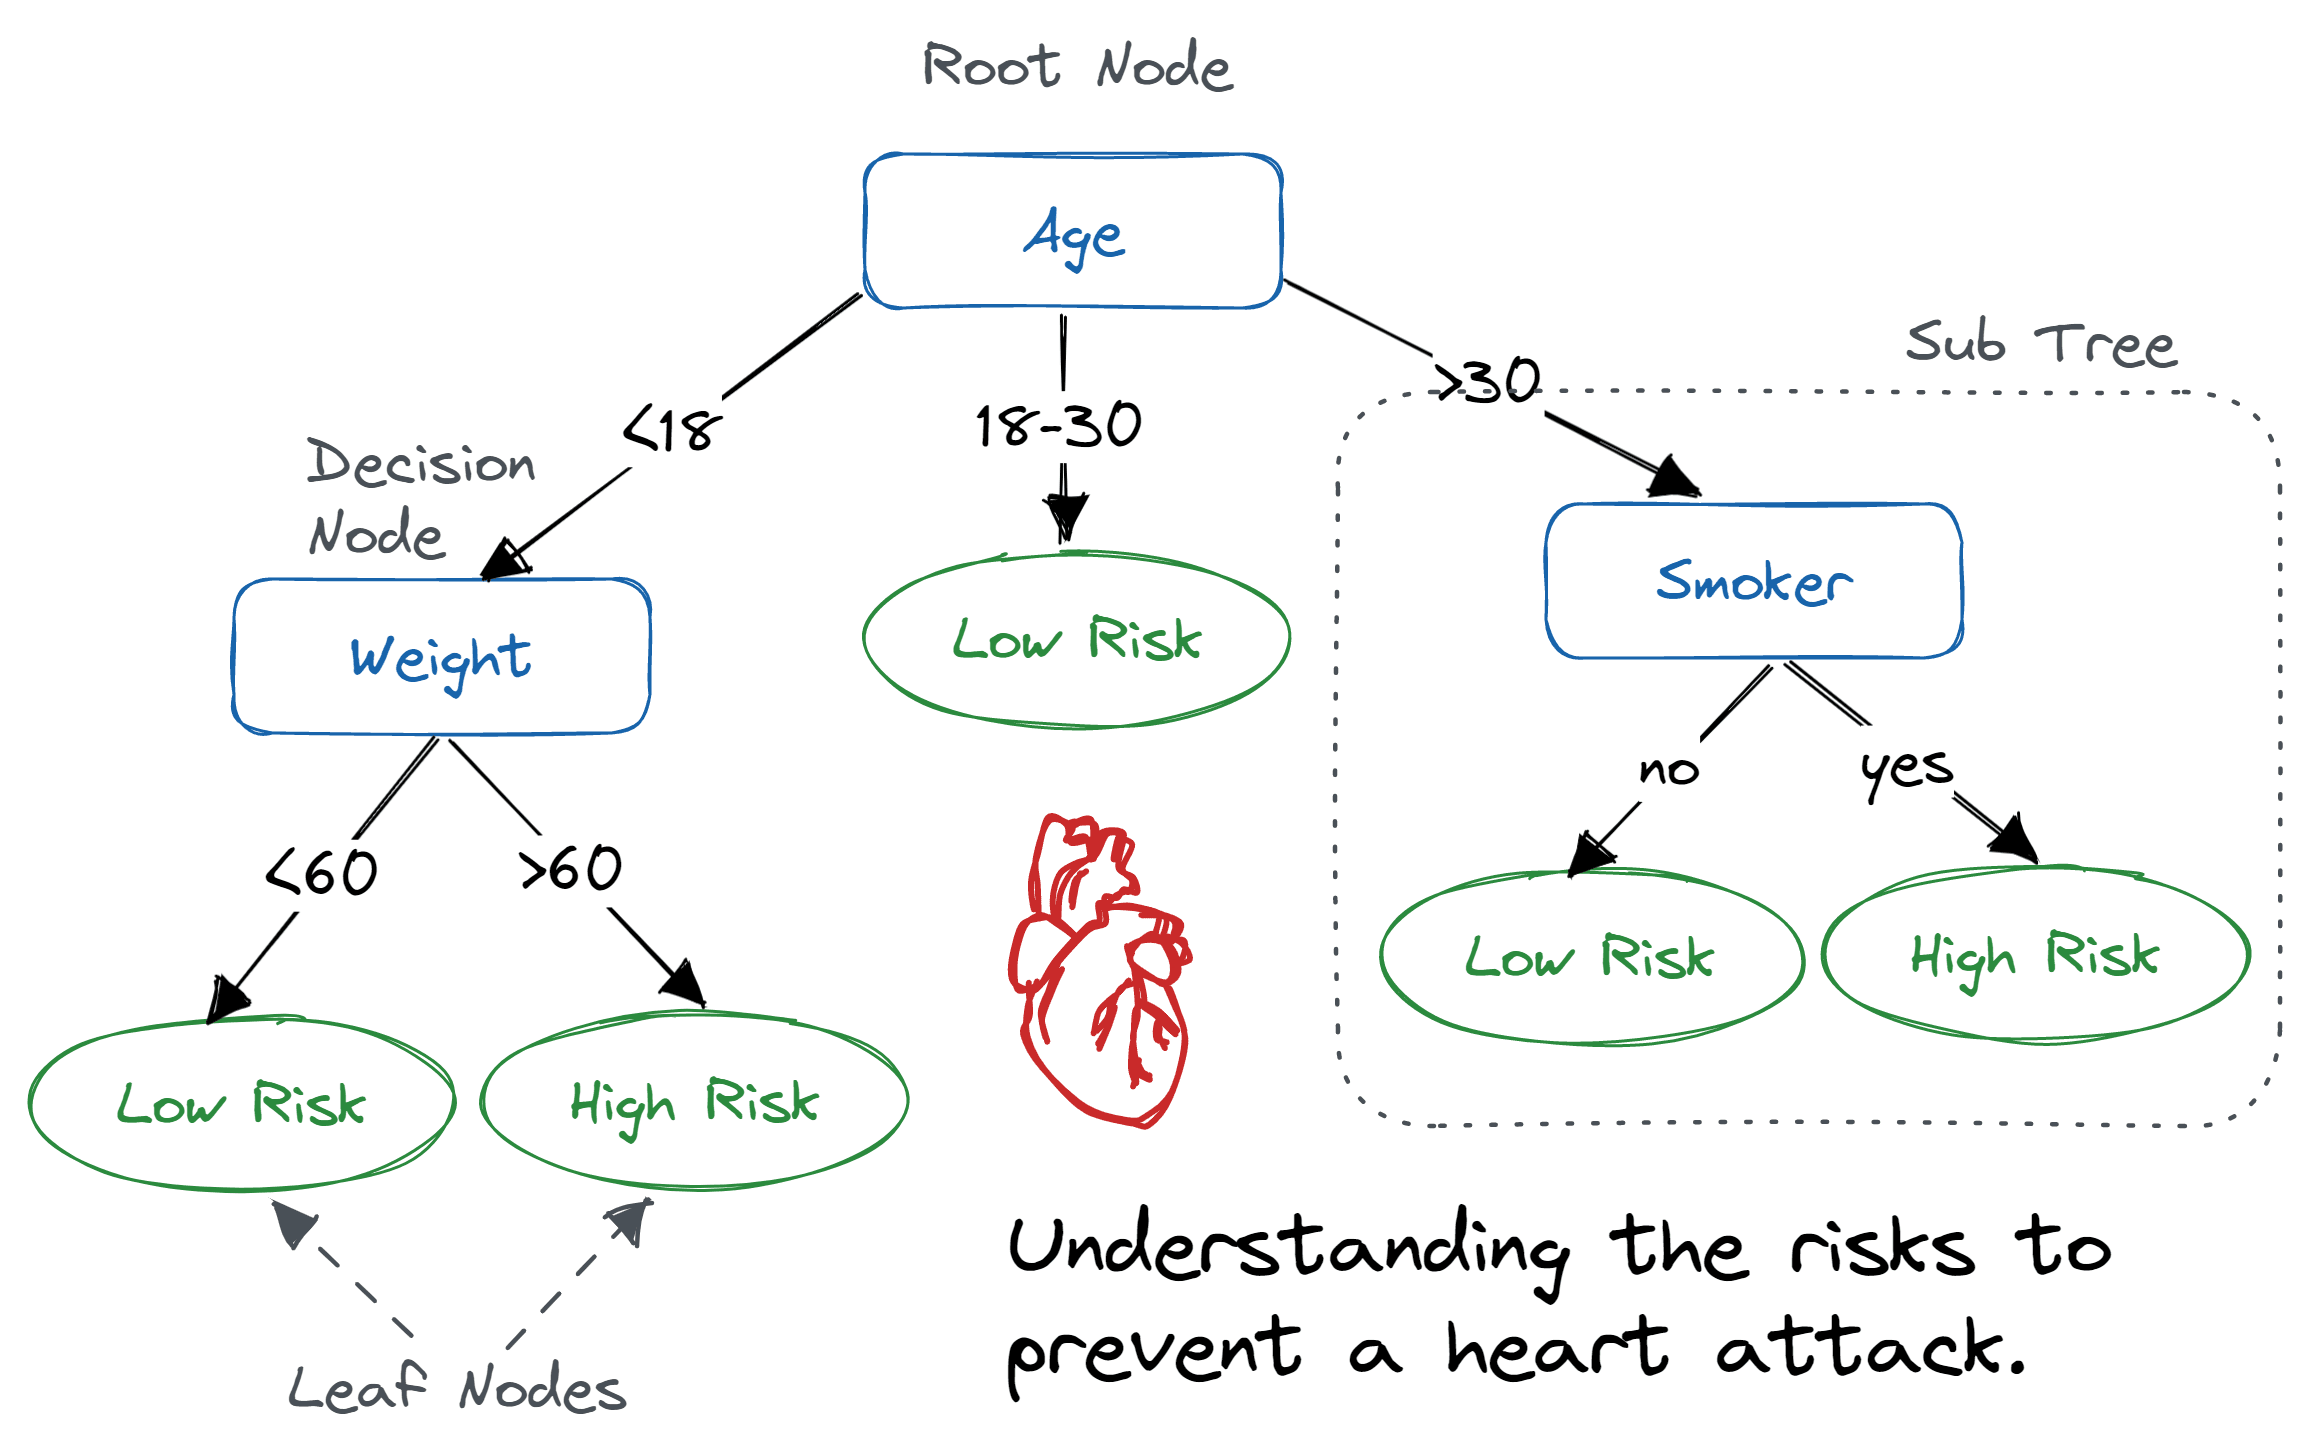
\includegraphics[width=0.9\textwidth]{./assets/images/decision_tree-examlpe.png}
	\caption{Decision Tree example}
\end{figure}
\subsection{Random Forests}
A random forest is an ensemble learning method that uses a collection of \textbf{decision trees} to make predictions. It builds multiple decision trees during training and outputs the class that is the mode of the classes (classification) or mean prediction (regression) of the individual trees.
\begin{figure}[h]
	\centering
	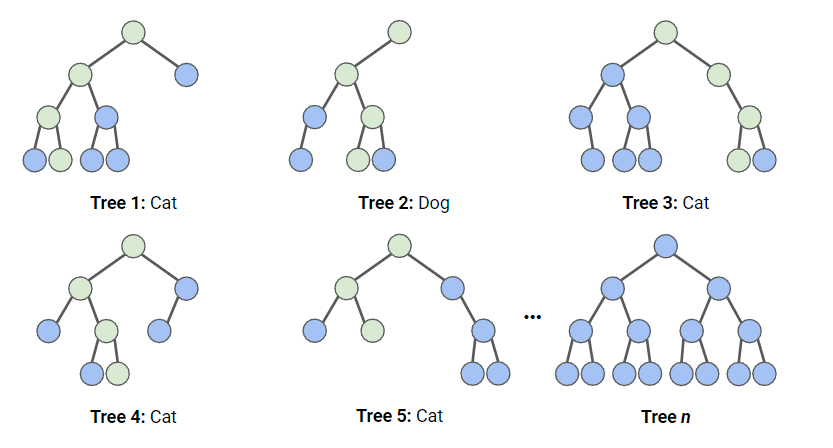
\includegraphics[width=0.9\textwidth]{./assets/images/Random forest.png}
	\caption{Random Forest}
\end{figure}

\section{Feature extraction and engineering}
\subsection{Feature extraction}
In this step, we extract relevant information from the \textbf{`pcap`} files to create a dataset suitable for machine learning.

Each entry in the dataset represents a network packet and contains attributes such as :

\begin{verbatim}
	["ip_source", "ip_destination", "frame_len", "protocol", "port_source",
	 "port_destination", "flags", "frame_number"]
\end{verbatim}
By converting the \textbf{pcap} files to \textbf{csv} format, we can easily analyze and process the data.

To manipulate packets in order to extract our features, we used \textbf{scapy}. Scapy is a powerful interactive packet manipulation library written in Python. It is able to forge or decode packets of a wide number of protocols, send them on the wire, capture them, match requests and replies.
\subsection{Feature engineering}
Because we cannot detect a DDoS attack by examining each individual row of our dataset alone, we reduced the size of our dataset by dividing it into batches of 100 rows. To do this, we calculated a series of statistical functions (such as mean, median, variance, standard deviation, etc.) for each batch using \textbf{pandas}. 

The results of these calculations will serve as the new rows in our dataset, effectively summarizing our previous data.

\section{Training the model}
To train our model, we used the \textbf{RandomForestClassifier} in scikit-learn. 
The RandomForestClassifier is a collection of decision trees. Each decision tree is built using a subset of the training data and a subset of the features.

To create each decision tree, the algorithm randomly selects a subset of the training data. 
Additionally, for each split in the decision tree, only a random subset of features is considered. This helps to introduce randomness into the trees and reduces the correlation between them.

The scikit-learn implementation of RandomForestClassifier uses an optimized version of the Random Forest algorithm to improve efficiency and scalability.
The algorithm supports parallelism, allowing it to take advantage of multi-core processors for faster training.

Our RandomForestClassifier constructor to create our Random Forest classifier model in scikit-learn with the following parameter:
n\_estimators: This parameter specifies the number of decision trees to be used in the Random Forest. For us we chose n\_estimators=10 wich means that the Random Forest will consist of 10 decision trees.
